\section{Theory behind the Faraday effect}
The \textit{Faradayeffect} refers to a megneto-optical phenomenon which can be explained in terms
of circular birefringence. The effect causes a rotation of the polarization direction with regards
to a applied magnetic field and its direction. It was discovered by \textit{faraday} in 1845 and
can be seen as the first experiment showing the interplay between light and electromagnetism. 
As already mentioned in the first part we can use the Maxwell equations to describe the magnetic
and electric field such that we can understand how the dielectricity of the material gives rise
to the phenomenon. For the experimental setup for seeing the faradayeffect you insert a medium,
which does not have to be optically active, between two polarizators. If we now fix the direction
of the magnetic field to be parallel to the direction of the incoming light we observe the 
already mentioned rotation.   
\subsection{Magneto-optic rotation}
As it turns out the first approximation the rotation angle of the polarization is proportional
to the Depth of the material $l$ and the magnetic field $B$:
\begin{equation}
    \alpha = V l B
\end{equation}
Where we introduced the Verdet-constant $V$. In the following we will derive this formula in order
to understand the physical nature of this constant \cite{staatsexamen}.
Lets assume without loss of generality a plane wave solution to the maxwell equation
with propagation in $z$-direction with speed v, 
entering the medium at $z=$, being turned with the angle
$\alpha = \phi  z$:
\begin{align}
x &= F \cos{(\phi z)} \cos{\left ( \omega \left ( t - \frac{z}{v} \right )\right)} \\ 
y &= F \sin{(\phi z)} \cos{\left ( \omega \left ( t - \frac{z}{v} \right )\right)}
\end{align}
if we now apply $\cos(\beta) = (e^{i\beta} + e^{-i\beta})/2$ 
(analogous $\sin(\beta) = (e^{i\beta} - e^{-i\beta})/2i$ )
and rename $\tau := (t-\frac{z}{v})$:
\begin{align}
x &= \frac{F}{4} \left (e ^{i\phi z} + e ^{-i\phi z} \right )
\left (e ^{i\omega \tau} + e ^{-i\omega \tau} \right ) \\ 
&= \frac{F}{2} \left ( \cos{(\phi z + \omega \tau)} + \cos{(\omega \tau -  \phi z )} \right ) \\
\Rightarrow y &= \frac{F}{2} \left ( \sin{(\phi z + \omega \tau)} - \sin{(\omega \tau -  \phi z )} \right )
\end{align}
which in particular shows how the linear polarized wave consists of two circular, reverse polarized
waves with relatives speeds:
\begin{align}
\frac{\omega}{v_+} &= \frac{\omega}{v} - \phi \label{eq:v+}\\ 
\frac{\omega}{v_-} &= \frac{\omega}{v} + \phi \label{eq:v-}
\end{align}
Subtracting these two equations yields
\begin{equation}
2\phi = \omega \left (\frac{1}{v_-} - \frac{1}{v_+} \right)
\end{equation}
which we can insert into the definition of $\alpha$ and the refraction index $n = c/v$:
\begin{align}
\alpha = \phi l &= \frac{\omega l}{2} \left (\frac{1}{v_-} - \frac{1}{v_+} \right) \\ 
 &= \frac{\omega l}{2c} \left (n_- - n_+ \right)
\end{align}
From equation \eqref{eq:v+} and \eqref{eq:v-} we get (implying for small $\phi$ in the last step):
\begin{equation}
v_{+/-} = \frac{\omega}{\frac{\omega}{v} \mp \phi} = \frac{v}{1 \mp \frac{\phi v}{\omega}} 
= v \left ( 1 \pm \frac{\phi v}{\omega}+ \left (\frac{\phi v}{\omega} \right)^2
\pm \left (\frac{\phi v}{\omega} \right)^3 + \left (\frac{\phi v}{\omega} \right)^4+ \cdots \right)
\approx v \left  (1 \pm \frac{\phi v}{\omega} \right )
\end{equation}
Using the semiclassical Bohrmodel we can understand the behavior of the electrons in 
first approximation with the Larmorfrequency:
\begin{equation}
\omega_L = \frac{-e B}{2 m c}
\end{equation}
Since the dynamics of the electrons is fundamentally connected to the dispersion of the material,
we can use this frequency to connect the Rotation of the polarization with the dynamical behavior 
of the electrons of the medium. If we go into a coordinatesystem which is rotating with $\omega_L$,
the electrons have their original frequency (predicted by the Bohr model), hence the electromagnetic
wave is shifted by this frequency with regards to the original coordinate system. Thus we get:
\begin{equation}
\alpha = \frac{\omega l}{2c} \left (n_{\omega + \omega_L} - n_{\omega - \omega_L}\right )  
\end{equation}
The refraction index in dependence of the frequency is given by the dispersion relation, which is 
dependent on the medium. For small frequencies we can taylor: 
\begin{equation}
n(\omega + \omega_L) \approx n(\omega) \pm \omega_L \frac{\partial n}{\partial \omega}
\end{equation}
and now we can write in this in terms of $\omega \frac{n}{w} = -\lambda \frac{n}{\lambda}$:
\begin{equation}
\alpha = \frac{\omega_L l \lambda}{c} \frac{\partial n}{\partial \lambda} = 
\frac{e l B \lambda}{2m c^2} \frac{\partial n}{\partial \lambda} \quad \text{Formula of Bequerel}
\end{equation}

\subsection{Half shade polarimeter}

\subsection{Experimental setup}
\begin{figure}
    \begin{centering}
        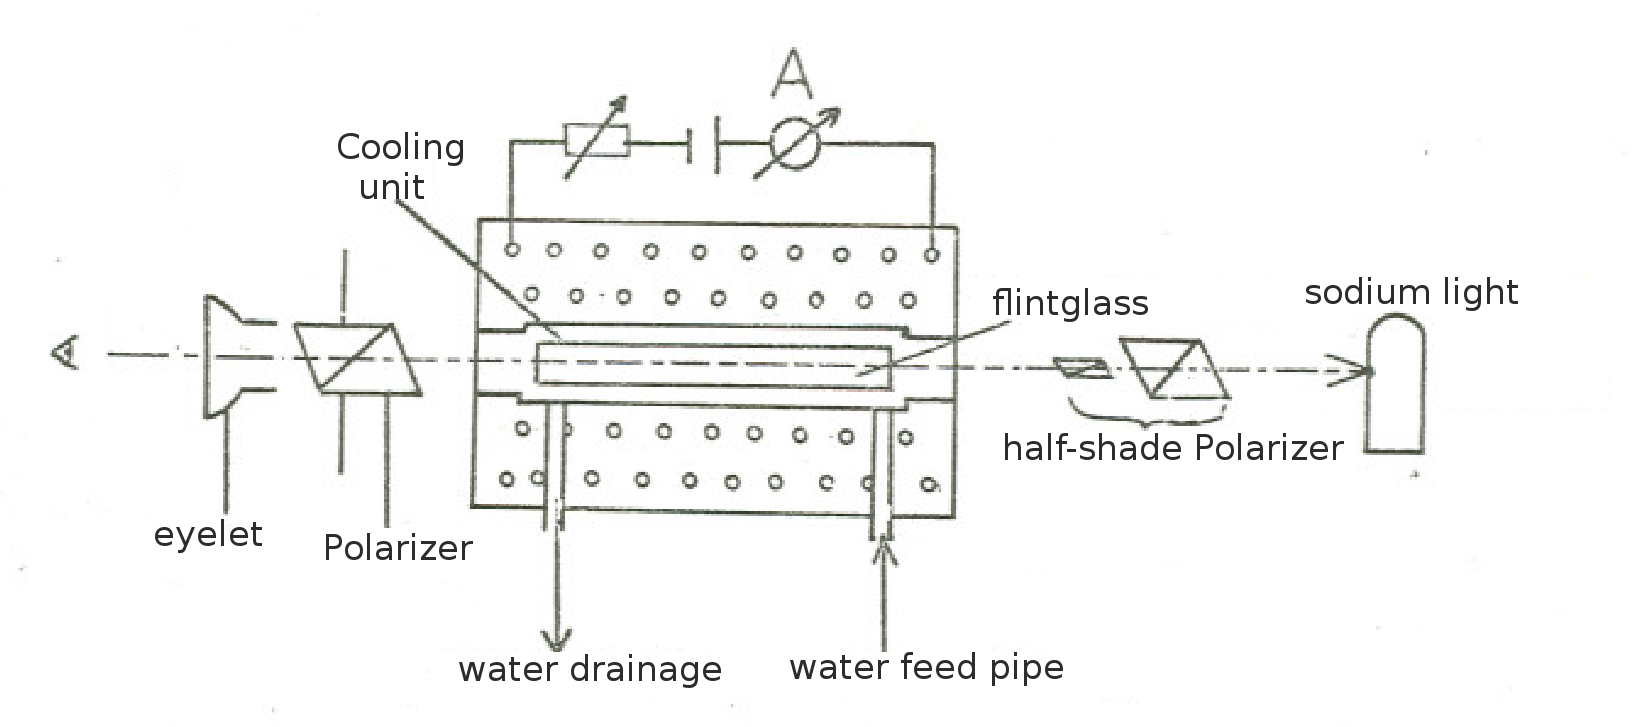
\includegraphics[width=18cm]{figures/faraday_setup2}
        \caption{Experimental setup (figure from \cite{staatsexamen}).}
        \label{fig:faraday_setup}
    \end{centering}
\end{figure}


\subsection{Method of measuring the rotation angle}

\subsection{Method of measuring angle between dirctions of polarization of half-shade polarimeter}
